\chapter{Metodología de diseño e implementación de recursos distribuidos}
\label{cap:metodologia}


\section{Especificación del tipo}

El primer paso que hay que hacer a la hora de crear un nuevo recurso en Puppet es definir el tipo de recurso. Para ello en un fichero habrá que especificar el nombre del nuevo tipo y los argumentos que éste tiene. Durante esta sección y la siguiente se usará el ejemplo de la arquitectura web de tres niveles. El primer motivo es que puede resultar más conocida que las infraestructuras de ejecución de trabajos. El segundo motivo es para demostrar que el enfoque que se ha tomado es lo suficientemente general y válido también para infraestructuras que nada tienen que ver con la ejecución de trabajos. \\

Una típica arquitectura de servicios web consta de al menos tres niveles: balanceo de carga, servidores web y base de datos. Cada uno de estos niveles está compuesto por al menos un elemento clave: el balanceador de carga, el servidor web y el servidor de base de datos, respectivamente. El balanceador de carga es el punto de entrada al sistema y el que se encarga, como su nombre indica, de repartir las peticiones de los clientes a los distintos servidores web. Los servidores web se encargan de servir las páginas web a los clientes y para ello, dependiendo de las peticiones que hagan los clientes, podrán leer o almacenar información en la base de datos. Para manipular dicha información los servidores web tendrán que comunicarse con el servidor de base de datos, que es el que hará efectiva la lectura y modificación de la información.\\

\begin{figure} [!htbp]
  \centering
  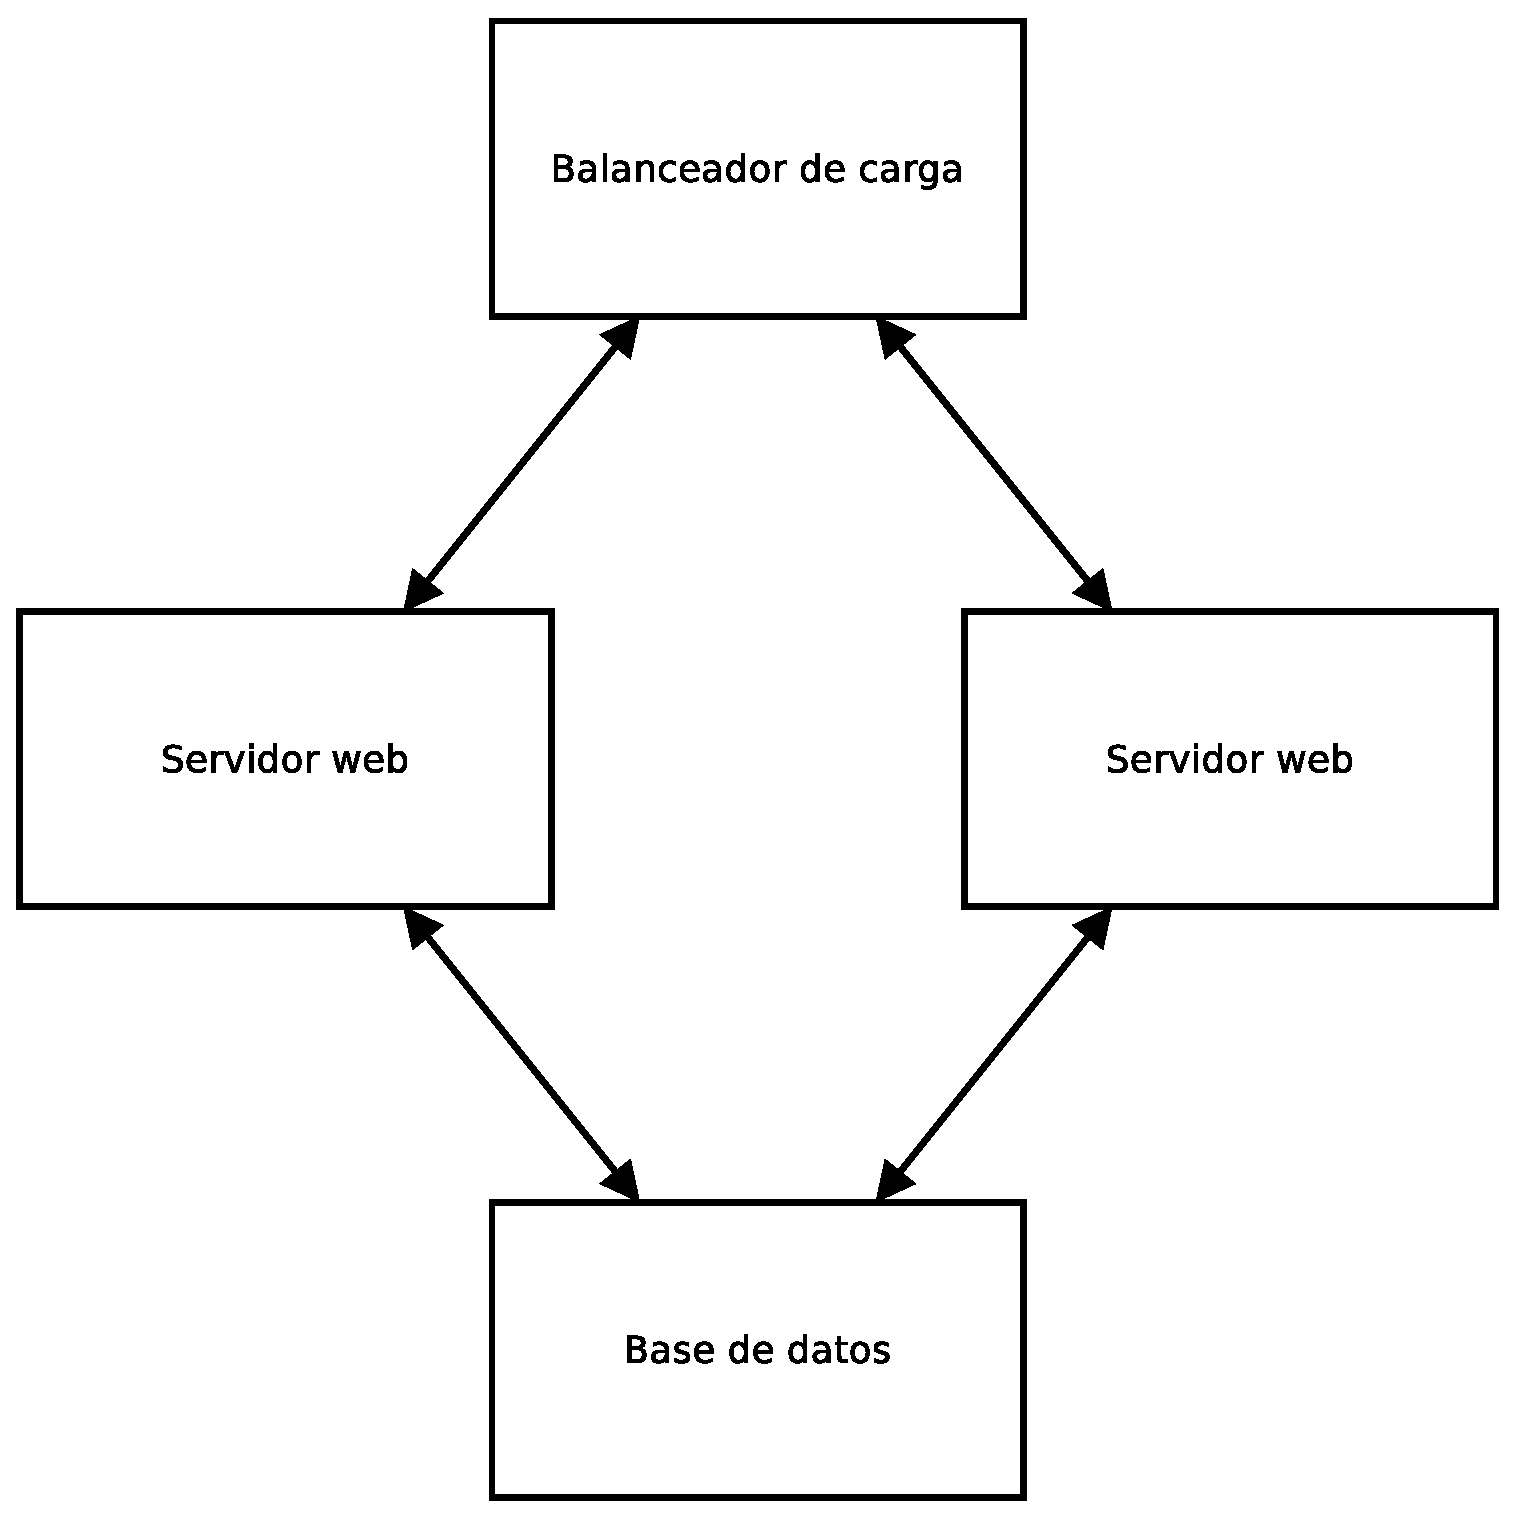
\includegraphics[width=0.5\textwidth]{figuras/Arquitectura_Web2.eps}
  \caption{Infraestructura web de tres niveles.}
\label{figure:arquitectura-web}
\end{figure}

La infraestructura usada como ejemplo consta de un balanceador de carga, dos servidores web y un servidor de bases de datos (Figura \ref{figure:arquitectura-web}).


La creación del tipo \texttt{web} se hace en el fichero \texttt{web.rb} (en el lugar apropiado dentro del correspondiente módulo) con un contenido similar a éste:

\begin{rubycode}
Puppet::Type.newtype(:web) do
   @doc = "Manages web clouds formed by KVM virtual machines."
   
   
   ensurable do

      desc "The cloud's ensure field can assume one of the following values:
   `running`: The cloud is running.
   `stopped`: The cloud is stopped.\n"
   
      newvalue(:stopped) do
         provider.stop
      end

      newvalue(:running) do
         provider.start
      end

   end


   # General parameters
   
   newparam(:name) do
      desc "The cloud name"
      isnamevar
   end
   
   newparam(:vm_domain) do
      desc "The XML file with the virtual machine domain definition. " +
           "Libvirt XML format must be used"
   end
   
   newproperty(:pool, :array_matching => :all) do
      desc "The pool of physical machines"
   end

   # ...


   # Web parameters
   
   newproperty(:balancer, :array_matching => :all) do
      desc "The balancer node's information"
   end
   
   newproperty(:server, :array_matching => :all) do
      desc "The server nodes' information"
   end
   
   newproperty(:database, :array_matching => :all) do
      desc "The database node's information"
   end

end

\end{rubycode}

Dentro del tipo \texttt{web}, los parámetros \texttt{name}, \texttt{vm\_domain} y \texttt{pool} se corresponden con los parámetros \texttt{Nombre}, \texttt{Fichero de dominio} y \texttt{Conjunto de máquinas físicas} definidos en la sección \ref{sec:modelado-puppet}. Los parámetros \texttt{balancer}, \texttt{server} y \texttt{database} son los parámetros propios de la arquitectura web.

Una vez que el tipo ya está definido, ya se puede ver cuál será el aspecto de un manifiesto para un recurso de tipo web:

\begin{lstlisting}
web {'mycloud':
   balancer => ["155.210.155.175", "/var/tmp/dceresuela/lucid-lb.img"],
   server => ["/etc/puppet/modules/web/files/server-ips.txt",
              "/etc/puppet/modules/web/files/server-imgs.txt"],
   database => ["155.210.155.177", "/var/tmp/dceresuela/lucid-db.img"],
   vm_domain => "/etc/puppet/modules/web/files/mycloud-template.xml",
   pool => ["155.210.155.70"],
   ensure => running,
}
\end{lstlisting}

%%%%%%%%%%%%%%%%%%%%%%%%%%%%%%%%%%%%%%%%%%%%%%%%%%%%%%%%%%%%%%%%%%%%%%%%%%%%%%%%
\section{Diseño e implementación del proveedor}

Una vez que se ha definido el tipo del recurso, queda definir el proveedor para ese tipo. En el caso de los recursos distribuidos, y teniendo en cuenta las funciones especificadas en la parte de \texttt{ensurable}, el proveedor deberá contener obligatoriamente las funciones \texttt{start} y \texttt{stop}. Un proveedor simplificado sería similar a éste:

\begin{rubycode}
Puppet::Type.type(:web).provide(:webp) do
   desc "Manages web clouds formed by KVM virtual machines"

   # Require files
   # ...

   # Makes sure the cloud is running.
   def start
   
      cloud = Cloud.new(CloudInfrastructure.new(), CloudLeader.new(), resource,
                        method(:err))
      puts "Starting cloud %s" % [resource[:name]]
      
      # Check existence
      if !exists?
         # Cloud does not exist => Startup operations
         
         # Check pool of physical machines
         puts "Checking pool of physical machines..."
         pm_up, pm_down = cloud.check_pool()
         unless pm_down.empty?
            puts "Some physical machines are down"
            pm_down.each do |pm|
               puts " - #{pm}"
            end
         end
         
         # Obtain the virtual machines' IPs
         puts "Obtaining the virtual machines' IPs..."
         vm_ips, vm_ip_roles, vm_img_roles = obtain_vm_data(cloud.resource)
         
         # Check whether you are one of the virtual machines
         puts "Checking whether this machine is part of the cloud..."
         part_of_cloud = vm_ips.include?(MY_IP)
         if part_of_cloud
            puts "#{MY_IP} is part of the cloud"
            
            # Check if you are the leader
            if cloud.leader?()
               cloud.leader_start("web", vm_ips, vm_ip_roles, vm_img_roles,
                                  pm_up, method(:web_monitor))
            else
               cloud.common_start()
            end
         else
            puts "#{MY_IP} is not part of the cloud"
            cloud.not_cloud_start("web", vm_ips, vm_ip_roles, vm_img_roles,
                                  pm_up)
         end
         
      else
         
         # Cloud exists => Monitoring operations
         puts "Cloud already started"
         
         # Check if you are the leader
         if cloud.leader?()
            cloud.leader_monitoring(method(:web_monitor))
         else
            puts "#{MY_IP} is not the leader"      # Nothing to do
         end
      end
      
   end


   # Makes sure the cloud is not running.
   def stop

      # ...
   
   end


   def status
      if File.exists?("/tmp/cloud-#{resource[:name]}")
         return :running
      else
         return :stopped
      end
   end
   
end
\end{rubycode}

Son especialmente importantes dentro de este proveedor las líneas 10, 30 y 40. En la línea 10 creamos un nuevo objeto de la clase \texttt{Cloud} (\ref{sec:modelado-framework}). En la línea 30 se llama a la función \texttt{obtain\_vm\_data} para obtener los datos de las máquinas virtuales (\ref{sec:modelado-framework}). En la línea 40 puede verse como el objeto de la clase \texttt{Cloud} se usa para llamar al método \texttt{leader\_start} que realizará las funciones de puesta en marcha como nodo líder del \emph{cloud} (\ref{sec:modelado-proveedor}). Uno de los parámetros de esa llamada es la función \texttt{web\_monitor} que se usará para monitorizar los aspectos particulares del \emph{cloud} web (\ref{sec:modelado-framework}).


%%%%%%%%%%%%%%%%%%%%%%%%%%%%%%%%%%%%%%%%%%%%%%%%%%%%%%%%%%%%%%%%%%%%%%%%%%%%%%%%
\section{Ejemplos de diseño e implementación}

En esta sección se verá cómo aplicar los pasos anteriores en las arquitecturas distribuidas AppScale y TORQUE.

%%%%%%%%%%%%%%%%%%%%%%%%%%%%%%%%%%%%%%%%%%%%%%%%%%%%%%%%%%%%%%%%%%%%%%%%%%%%%%%%
\subsection{Diseño e implementación de un recurso distribuido para una infraestructura AppScale}

Una infraestructura AppScale puede ser definida de dos maneras: mediante un despliegue por defecto o uno personalizado. En un despliegue por defecto un nodo es el encargado de controlar la infraestructura y el resto de nodos se encargan de hacer el resto del trabajo. En un despliegue personalizado podemos especificar con mayor grado de precisión qué tipo de trabajo debe hacer cada nodo. Por ejemplo, podemos indicar qué nodos se encargarán de alojar las aplicaciones de los usuarios, qué nodos alojarán la base de datos o qué nodos serán los encargados de ejecutar los trabajos de computación. Para administrar una infraestructura AppScale, sin importar el tipo de despliegue, necesitaremos una cuenta de correo y una contraseña. Este usuario y contraseña son necesarios para poder administrar las aplicaciones alojadas y observar el estado de la infraestructura. \\

En un despliegue por defecto los posibles roles que puede tomar un nodo son:

\begin{description}
\item[\texttt{controller}]: La máquina que desempeñará el rol de nodo controlador.
\item[\texttt{servers}]: La lista de máquinas que desempeñarán el rol de nodos de trabajo.
\end{description}

Mientras que los posibles roles que puede desempeñar un nodo en un despliegue personalizado y que resultan interesantes desde nuestro punto de vista son:

\begin{description}
\item[\texttt{master}]: La máquina que desempeñará el rol de nodo maestro.
\item[\texttt{appengine}]: Los servidores para alojar las aplicaciones.
\item[\texttt{database}]: Las máquinas que contienen la base de datos.
\item[\texttt{login}]: La máquina encargada de redirigir a los usuarios a sus servidores. Es también la que se le facilita al administrador de la infraestructura para que realice las tareas administrativas.
\item[\texttt{open}]: Las máquinas de ejecución de trabajos. También pueden ser usadas como nodos de reserva por si falla algún otro nodo.
\end{description}

El tipo \texttt{appscale} deberá ser capaz de soportar ambos tipos de despliegue. Además de los parámetros necesarios para los roles de las máquinas, también debe contar con la cuenta de correo y la contraseña para el administrador del \emph{cloud}. Los parámetros del tipo \texttt{appscale} son:

\begin{rubycode}
Puppet::Type.newtype(:appscale) do
   @doc = "Manages AppScale clouds formed by KVM virtual machines."
   
   # ...

   # AppScale parameters
   
   newproperty(:controller, :array_matching => :all) do
      desc "The controller node"
   end

   newproperty(:servers, :array_matching => :all) do
      desc "The server nodes"
   end


   newproperty(:master, :array_matching => :all) do
      desc "The master node"
   end

   newproperty(:appengine, :array_matching => :all) do
      desc "The appengine nodes"
   end

   newproperty(:database, :array_matching => :all) do
      desc "The database nodes"
   end

   newproperty(:login, :array_matching => :all) do
      desc "The login node"
   end

   newproperty(:open, :array_matching => :all) do
      desc "The open nodes"
   end

   newproperty(:zookeeper, :array_matching => :all) do
      desc "The zookeeper nodes"
   end

   newproperty(:memcache, :array_matching => :all) do
      desc "The memcache nodes"
   end
   

   newparam(:app_email) do
      desc "AppScale administrator e-mail"
      defaultto "david@gmail.com"
   end
   
   newparam(:app_password) do
      desc "AppScale administrator password"
      defaultto "appscale"
   end

end
\end{rubycode}

Hay multitud de despliegues posibles combinando estos roles, pero será de especial interés el que permite ejecutar trabajos de computación en AppScale (Figura \ref{figure:arquitectura-appscale}).

\begin{figure} [!htbp]
  \centering
  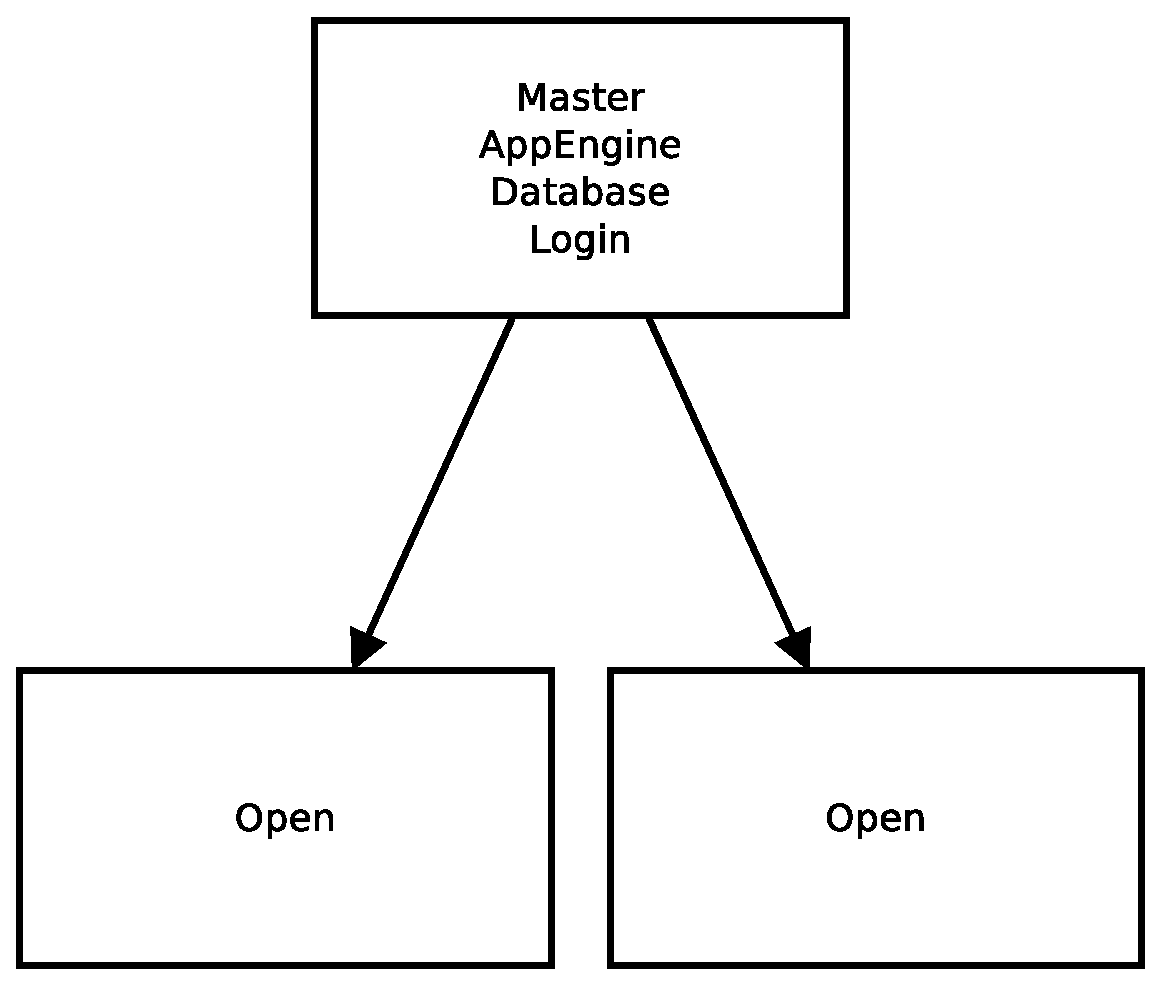
\includegraphics[width=0.5\textwidth]{figuras/Arquitectura_AppScale.eps}
  \caption{Infraestructura AppScale en despliegue personalizado.}
\label{figure:arquitectura-appscale}
\end{figure}

Para lograr un despliegue de este tipo podría utilizarse un manifiesto similar a éste:

\begin{lstlisting}
appscale {'mycloud':
   master    => ["155.210.155.73",
                 "/var/tmp/dceresuela/lucid-tor1.img"],
   appengine => ["155.210.155.73",
                 "/var/tmp/dceresuela/lucid-tor1.img"],
   database  => ["155.210.155.73",
                 "/var/tmp/dceresuela/lucid-tor1.img"],
   login     => ["155.210.155.73",
                 "/var/tmp/dceresuela/lucid-tor1.img"],
   open      => ["/etc/puppet/modules/appscale/files/open-ips.txt",
                 "/etc/puppet/modules/appscale/files/open-imgs.txt"],
   vm_domain => "/etc/puppet/modules/appscale/files/mycloud-template.xml",
   pool => ["155.210.155.70"],
   ensure => running,
}
\end{lstlisting}


%%%%%%%%%%%%%%%%%%%%%%%%%%%%%%%%%%%%%%%%%%%%%%%%%%%%%%%%%%%%%%%%%%%%%%%%%%%%%%%%
\subsection{Diseño e implementación de un recurso distribuido para una infraestructura TORQUE}

Una infraestructura TORQUE está formada por un nodo maestro y un conjunto de nodos de computación (Figura \ref{figure:arquitectura-torque}). El nodo maestro es el encargado de recibir los trabajos a ejecutar y de asegurar una correcta planificación para esos trabajos; en su versión más simple el planificador es una cola FIFO. Los nodos de computación son los encargados de ejecutar los trabajos enviados por el nodo maestro y, una vez terminados, enviarle los resultados de vuelta. \\

\begin{figure} [!htbp]
  \centering
  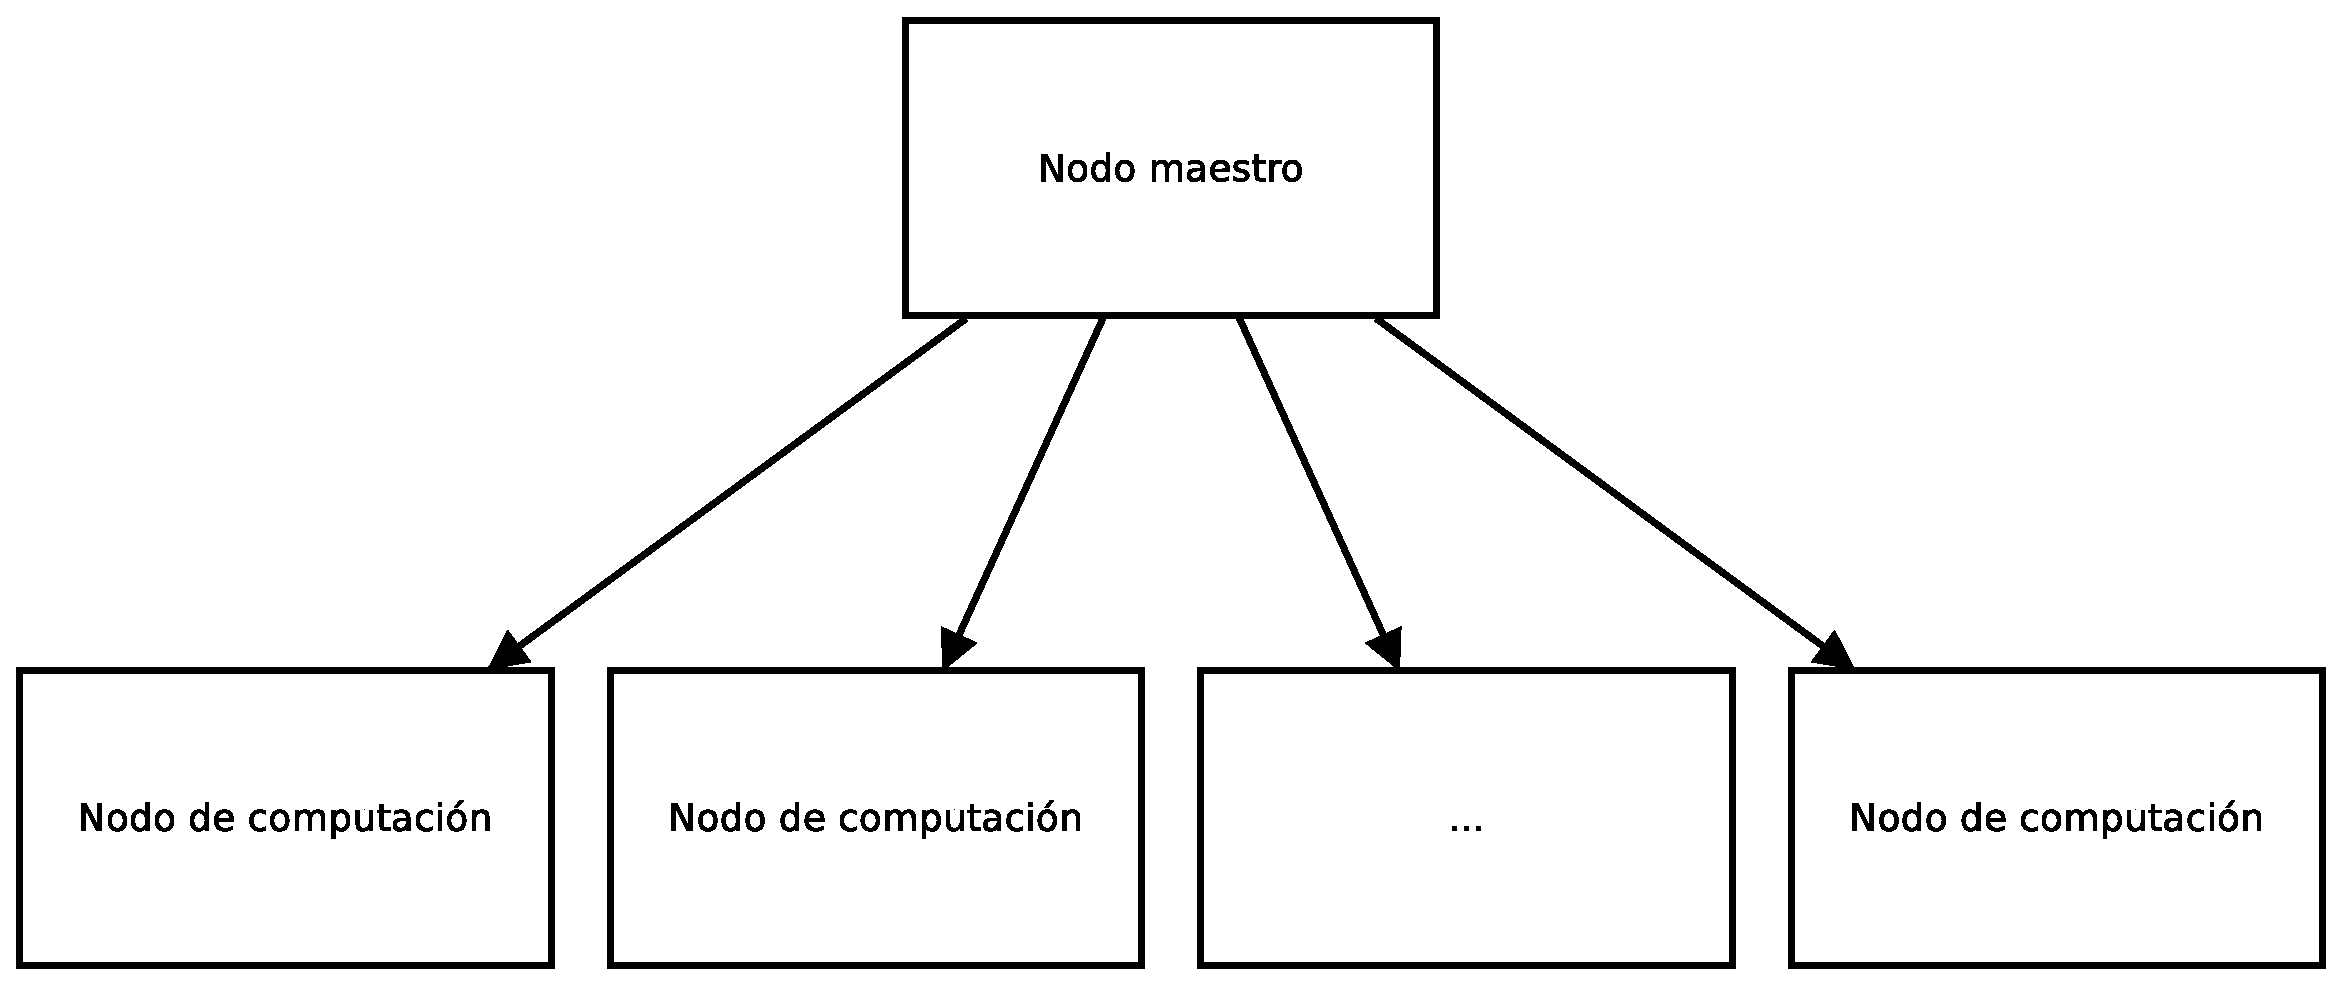
\includegraphics[width=13.5cm]{figuras/Arquitectura_Torque.eps}
  \caption{Infraestructura Torque.}
\label{figure:arquitectura-torque}
\end{figure}

Los nuevos parámetros que aparecen en el tipo \texttt{torque} reflejan esta nueva infraestructura:

\begin{rubycode}
Puppet::Type.newtype(:torque) do
   @doc = "Manages Torque clouds formed by KVM virtual machines."
   
   # ...

   # Torque parameters
   newproperty(:head, :array_matching => :all) do
      desc "The head node's information"
   end
   
   newproperty(:compute, :array_matching => :all) do
      desc "The compute nodes' information"
   end
   
end
\end{rubycode}

La sintaxis del manifiesto de puesta en marcha también se modifica para reflejar este cambio. Un ejemplo para la puesta en marcha de una infraestructura TORQUE sería similar a éste:

\begin{lstlisting}
torque {'mycloud':
   head => ["155.210.155.73", "/var/tmp/dceresuela/lucid-tor1.img"],
   compute => ["/etc/puppet/modules/torque/files/compute-ips.txt",
               "/etc/puppet/modules/torque/files/compute-imgs.txt"],
   vm_domain => "/etc/puppet/modules/torque/files/mycloud-template.xml",
   pool => ["155.210.155.70"],
   ensure => running,
}
\end{lstlisting}

Por otro lado, un posible manifiesto de parada sería similar a éste:

\begin{lstlisting}
torque {'mycloud':
   head => ["155.210.155.73", "/var/tmp/dceresuela/lucid-tor1.img"],
   compute => ["/etc/puppet/modules/torque/files/compute-ips.txt",
               "/etc/puppet/modules/torque/files/compute-imgs.txt"],
   pool => ["155.210.155.70"],
   ensure => stopped,
}
\end{lstlisting}


